%!TEX root = ../thesis.tex
\chapter{Introduction}

%!TEX root = ../../thesis.tex

\section{Overview}

Developing a text editor in a browser environment differs from implementing a text editor in a desktop environment. Any implementation is based on the features of the browsers. Development is generally restricted to the components and APIs offered by the HTML5 standard as well as experimental features that are usually implemented in a subset of browsers\footnote{Whether a specific component or API can be used or not, is determined by the intended audience and browser market share.}. The boundaries of these restrictions can be overcome. It is common practice to combine native elements and APIs in ways they have not been designed for to enable features that are not offered. These techniques are often referred to as ''hacks'' and, despite this terminology, are generally not regarded as a bad practice.

This chapter will discuss the basics of plain-text and rich-text editing in browsers as well as the APIs and techniques that are natively offered.%as well as the specifics of implementing a rich-text editor in the browser without the use of hacks.

% by modern web browsers

%\footnote{Native to the browser, not the operating system.}

%This chapter will describe the basics of text and rich-text editing in browsers as well as the APIs and techniques used. The origins and the history of rich-text editing pose the question if the paradigms rich-text editing is based on have been thoroughly reviewed and if alternative ways for an implementation, possibly using hacks, could be considered.

% When not using third-party plugins like Adobe Flash or Microsoft Silverlight, development is restricted to the components and APIs


\part{Theory}
\label{part:theory}

\chapter{Text editing in desktop environments}
\label{ch:desktop}

%!TEX root = ../thesis.tex

\section{Basics of plain-text editing} % word-processing

caret
selection
input

\section{Basics of rich-text editing} % word-processing

document tree
formatting algorithms

% we will see that contenteditable handles all this, but in my solution this all needs to be coded again
% I need to discuss that the benefits are bigger than having to do this

\section{Libraries for desktop environments}

It is no longer needed to implement basic rich-text editing components from the ground up. Rich-text editing has become a standard and most modern Frameworks, system APIs or GUI libraries come with built-in capabilities. Table \ref{table:rich-text-components-desktop} lists rich-text text components for popular languages and frameworks.

\begin{table}[]
\centering
\begin{tabular}{ll}
\hline
Environment & Component \\ \hline
Java (Swing) & JTextPane / JEditorPane \\
MFC & CRichEditCtrl \\
Windows Forms / .NET & RichTextBox \\
Cocoa & NSTextView \\
Python & Tkinter Text \\
Qt & QTextDocument \\ \hline
\end{tabular}
\caption{Rich-text components in desktop environments}
\label{table:rich-text-components-desktop}
\end{table}

\chapter{Text editing in browser environments}
\label{ch:browser}

%!TEX root = ../../thesis.tex

\section{Overview}

Developing a text editor in a browser environment differs from implementing a text editor in a desktop environment. Any implementation is based on the features of the browsers. Development is generally restricted to the components and APIs offered by the HTML5 standard as well as experimental features that are usually implemented in a subset of browsers\footnote{Whether a specific component or API can be used or not, is determined by the intended audience and browser market share.}. The boundaries of these restrictions can be overcome. It is common practice to combine native elements and APIs in ways they have not been designed for to enable features that are not offered. These techniques are often referred to as ''hacks'' and, despite this terminology, are generally not regarded as a bad practice.

This chapter will discuss the basics of plain-text and rich-text editing in browsers as well as the APIs and techniques that are natively offered.%as well as the specifics of implementing a rich-text editor in the browser without the use of hacks.

% by modern web browsers

%\footnote{Native to the browser, not the operating system.}

%This chapter will describe the basics of text and rich-text editing in browsers as well as the APIs and techniques used. The origins and the history of rich-text editing pose the question if the paradigms rich-text editing is based on have been thoroughly reviewed and if alternative ways for an implementation, possibly using hacks, could be considered.

% When not using third-party plugins like Adobe Flash or Microsoft Silverlight, development is restricted to the components and APIs

%!TEX root = ../../thesis.tex
\section{Plain-text editing}

Text input components for browsers have been introduced with the specification of HTML 2.0\footnote{\url{https://tools.ietf.org/html/rfc1866}, last checked on 07/15/2015}. The components proposed include inputs for single line (written as \code{<input type="text" />}) and multiline texts (written as \code{<textarea></textarea>}). These inputs allow writing plain-text only.

%!TEX root = ../../thesis.tex
\section{Rich-text editing}

Major browsers, i.e. any browser with a market share above 0.5\%\cite{ag}, do not offer native input fields that allow rich-text editing. Neither the W3C's HTML5 and HTML5.1 specifications nor the WHATWG HTML specification recommend such elements. However, by being able to display HTML, browsers effectively are rich-text viewers. By the early 2000s, the first JavaScript libraries emerged, that allowed users to interactively change (parts of) a website to enable rich-text editing in the browser. The techniques used will be discussed in section~\ref{sec:html-editing-apis} through section~\ref{sec:useage-of-html-editing-apis}.

% \footnote{\url{http://gs.statcounter.com/#all-browser-ww-monthly-201406-201506-bar}, last checked on 07/15/2015}
%!TEX root = ../../thesis.tex
\section{HTML Editing APIs}
\label{sec:html-editing-apis}

In July 2000, with the release of Internet Explorer 5.5, Microsoft introduced the IDL attributes\footnote{IDL attributes can only be set to DOM objects via JavaScript, whereas content attributes can be set to tags in the HTML source code. See \url{http://www.w3.org/TR/WebIDL/}, last checked on 08/17/2015} \texttt{contentEditable} and \texttt{designMode} along with the content attribute \texttt{contenteditable}\footnote{\url{https://msdn.microsoft.com/en-us/library/ms533720(v=vs.85).aspx}, last checked on 07/10/2015}\footnote{\url{https://msdn.microsoft.com/en-us/library/ms537837(VS.85).aspx}, last checked on 07/10/2015}. These attributes were neither part of the W3C's HTML 4.01 specifications\footnote{\url{http://www.w3.org/TR/html401/}, last checked on 07/14/2015} nor the ISO/IEC 15445:2000\footnote{\url{http://www.iso.org/iso/iso\_catalogue/catalogue\_tc/catalogue\_detail.htm?csnumber=27688}, last checked on 07/14/2015}, the defining standards of that time. Table \ref{table:editing-api-attributes} lists these attributes and possible values.

% Please add the following required packages to your document preamble:
% \usepackage{graphicx}
\begin{table}[]
\centering
\resizebox{\textwidth}{!}{%
\begin{tabular}{llll}
\hline
Attribute       & Type              & Can be set to         & Possible values                     \\ \hline
designMode      & IDL attribute     & Document              & "on", "off"                         \\
contentEditable & IDL attribute     & Specific HTMLElements & boolean, "true", "false", "inherit" \\
contenteditable & content attribute & Specific HTMLElements & empty string, "true", "false"       \\ \hline
\end{tabular}
}
\caption{Editing API attributes}
\label{table:editing-api-attributes}
\end{table}

\begin{lstlisting}[language=html, caption=An element set to editing mode, label=lst:div-contenteditable]
<div contenteditable="true">
  This text can be edited by the user.
</div>
\end{lstlisting}

By setting \texttt{contenteditable} or \texttt{contentEditable} to ''true'' or \texttt{designMode} to ''on'', Internet Explorer 5.5 switches the affected elements and their children to an editing mode. The \texttt{designMode}-attribute can only be applied to the entire document and the \texttt{contentEditable} and \texttt{contenteditable} attributes can be applied to specific HTML elements as described on Microsoft's Developer Network (MSDN) online documentation\footnote{\url{https://msdn.microsoft.com/en-us/library/ms537837(VS.85).aspx}, last checked on 07/10/2015}. These elements include ''divs'', ''paragraphs'' and the document's ''body'' element amongst others. Other than that, there is no difference in these attributes. In editing mode

\begin{enumerate}
\item Users can interactively click on and type inside texts
\item An API providing commands for editing text is enabled that can be accessed via JScript and JavaScript
\end{enumerate}

When an element is switched to editing mode, the browser handles setting the caret if a user clicks inside the text, accepting keyboard input and modifying text nodes entirely by itself. No further scripting is necessary.

The API enabled by the editing mode must be called globally on the \texttt{document} object, but will only execute when the user's selection or caret is contained within an element in editing mode. Table \ref{table:editing-mode-api} lists the full HTML editing API. To format text, the method \texttt{document.execCommand} must be used.

\begin{lstlisting}[language=JavaScript, caption=Emphasizing text using the HTML editing API, label=lst:execcommand-italics]
document.execCommand('italic', false, null);
\end{lstlisting}

\reflisting{lst:execcommand-italics} demonstrates an example call of the ''italic'' command. Calling this at any time on the \code{document} object, the browser will wrap the currently selected text (if inside an element in editing mode) with \code{<i>} tags. The method accepts three parameters.

% Please add the following required packages to your document preamble:
% \usepackage{graphicx}
\begin{table}[]
\centering
\resizebox{\textwidth}{!}{%
\begin{tabular}{llll}
\hline
Order       & Parameter              & Description \\ \hline
1 & cmdID & The name of the command that will be executed \\
2 & showUI & Determines if the browser will display a dialog if needed \\
2 & value & A parameter that can be passed to the command invoked with the cmdID \\ \hline
\end{tabular}
}
\caption{execCommand parameters}
\label{table:execcommand_parameters}
\end{table}


The first parameter is the ''Command Identifier'', which determines which command to execute. This can be ''italic'' to italicize the current selection or ''createLink'' to create a link with the currently selected text as label.

\begin{lstlisting}[language=JavaScript, caption=Creating a link using the HTML editing API, label=lst:execcommand-link]
document.execCommand('createLink', false, 'http://example.com/');
\end{lstlisting}

The \textit{third} parameter will be passed on to the internal command\footnote{The command invoked using the command identifier} as a parameter. In the case of a \texttt{createLink} command, the third parameter is the URL to be used for the link to create. The \textit{second} parameter determines if executing a command should display a user interface specific to the command. Using the \texttt{createLink} command with the second parameter set to \texttt{true} while not passing a third parameter, the user will be prompted with a system dialog to enter a URL. Most commands (command identifiers) \code{execCommand} accepts trigger text formatting. This includes commands to format text as bold, underlined, struck-through or as a headline. A full list of possible command identifiers can be found on MSDN\footnote{\url{https://msdn.microsoft.com/en-us/library/ms533049(v=vs.85).aspx}, last checked on 07/10/2015}. Apart from executing commands, the API enabled by the editing mode includes the functions \code{queryCommandEnabled}, \code{queryCommandIndeterm}, \code{queryCommandState}, \code{queryCommandSupported} and \code{queryCommandValue} which allow reading attributes related to the editing mode. % A full description of these commands can be found in \reftable{table:editing_mode_api}.




%\section{Web-based rich-text editors}

\section{Usage of HTML Editing APIs for rich-text editors}
\label{sec:useage-of-html-editing-apis}

%\begin{figure}[!htb]
%\centering
%\makebox[\textwidth]{\includegraphics[width=0.5\textwidth]{images/editingmode_usage.pdf}}
%\caption{Usage of HTML editing APIs to implement rich-text editors}
%\label{fig:formatting_dom_tree}
%\end{figure}

\begin{figure}
\centering
%\begin{subfigure}{.5\textwidth}
%  \centering
  \includegraphics[width=.4\linewidth]{images/ckeditor-demo-overlayed.png}
%  \caption{A subfigure}
%  \label{fig:sub1}
%\end{subfigure}%
%\begin{subfigure}{.5\textwidth}
%  \centering
  \includegraphics[width=.4\linewidth]{images/tinymce-demo-overlayed.png}
%  \caption{A subfigure}
%  \label{fig:sub2}
%\end{subfigure}
\caption{Usage of HTML editing APIs in CKEditor and TinyMCE}
\label{fig:usage_contenteditable_screenshots}
\end{figure}


Most web-based rich-text editors use HTML editing APIs as their basis. The popular editors ''CKEditor'' and ''TinyMCE'' dynamically create an \texttt{iframe} on instantiation and set its \texttt{body} to editing mode using the \texttt{contenteditable}-attribute. This way, users can type inside the \code{iFrame} which acts as a text input field. Both libraries wrap the \texttt{iframe} in a user interface with buttons to format the \texttt{iframe}'s contents. Using the interface, the commands of \texttt{document.execCommand} will be called on the \texttt{iframe}'s \texttt{document} and the selected text will be formatted. While using an \texttt{iframe} is still in practice, many newer editors use a  \texttt{div} element instead. The user interfaces vary between different editors. %Some editors do not show any chrome unless text will be selected

Usually, rich-text editors implemented this way wrap their editing capabilities, including \texttt{document.execCommand}, in an API to enrich functionality and provide higher-level concepts. As discussed in \refpart{part:discussion}, using HTML editing APIs requires a lot of workarounds, which some editors account for in the implementation of their library. Rich-text editing libraries can been downloaded JavaScript files and included in a web project. To display an editor on a website, it is common to select a \code{textarea} element on the website, that the library will replace with the rich-text editor. To integrate the editor into web forms, most libraries will mirror their contents to the selected \code{textarea}, so they can be submitted to a server.

For years, the market of web-based rich-text editors has been dominated by ''CKEditor'' and ''TinyMCE''. Both editors remain among the most popular choices. In the last years, the number of editors increased drastically. Popular choices on GitHub, rated by the number of ''stars'', include ''MediumEditor'', ''wysihtml'' and ''Summernote''. As Piotrek Koszuli\'{n}ski points out, most editors ''really doesn't[sic] work''\cite{bj} for the reasons discussed in \refsection{sec:disadvantages_of_html_editing_apis}.

%\textit{Should I elaborate this a bit more?}

%!TEX root = ../../thesis.tex
\chapter{Overview}
% \section{History and origins of HTML Editing APIs}

%HTML editing APIs have been poorly designed. Sections V to W discuss the origins and the reasons why HTML editing APIs have been standardized and are supported by all major browser. It can be seen, that they did not came to be because of their good design. In sections X and Y will discuss the design of these APIs.

% !!!



HTML editing APIs are the standard and the recommended way by the W3C and the WHATWG for implementing rich-text editors on the web. However, its implementations across major web browsers are inconsistent, known to contain numerous bugs and have a limited and imprecise API.

Understanding the origins and the history of rich-text editing on the web poses the question if the paradigms it is based on have been thoroughly reviewed and if alternative ways for an implementation, possibly using hacks, should be considered.

\refchapter{ch:editing_apis_history} will discuss the history and origins of HTML editing APIs. \refchapter{ch:editing_apis_adv_disadv} will discuss its advantages and disadvantages and
\refchapter{ch:editing_apis_alt} will discuss possible alternatives.

%This section will discuss the origins and adaption of HTML editing APIs as well as its advantages, disadvantages and alternatives.




%However, they are full of bugs and have caused companies like Google, Microsoft and Apple and its downsides have been discussed by companies like Google and Medium.

%creates unpredictable markup
%its API is limited and imprecise
%!TEX root = ../../thesis.tex


\section{Browser support}
\label{sec:edit_apis_browser_support}
%% \section{Development of HTML Editing APIs}

As discussed in \refsection{sec:html-editing-apis} HTML editing APIs have been introduced in July 2000 with the release of Internet Explorer 5.5 by Microsoft and have not been part of any standard of that time.

%With the release of Internet Explorer 5.5 and 

With the introduction of editing capabilities, Microsoft released a short documentation\footnote{\url{https://msdn.microsoft.com/en-us/library/ms537837(VS.85).aspx}, last checked on 07/10/2015}, containing the attributes' possible values and element restrictions along with two code examples. Although a clear purpose has not been stated, the code examples demonstrated how to implement rich-text input fields with it. Mark Pilgrim, author of the ''Dive into'' book series and contributor to the the WHATWG, states that the API's first use case has been for rich-text editing\footnote{\url{https://blog.whatwg.org/the-road-to-html-5-contenteditable}, last checked on 07/10/2015}. 

%% With the release of Internet Explorer 5.5 and the introduction of editing capabilities, Microsoft released a sparse documentation\footnote{\url{https://msdn.microsoft.com/en-us/library/ms537837(VS.85).aspx}, last checked on 07/10/2015} describing only the availability and the before-mentioned element restrictions of these attributes. 

%% According to Mark Pilgrim, author of the ''Dive into'' book series and contributor to the the Web Hypertext Application Technology Working Group (WHATWG),, but its first use case has been for rich-text editing\footnote{\url{https://blog.whatwg.org/the-road-to-html-5-contenteditable}, last checked on 07/10/2015}. 

% It is notable, that the available command identifiers mostly include text-editing (or related) commands, but not exclusively. Other commands include navigating to other URLs or controlling the browser's cache.

In March 2003, the Mozilla Foundation introduced an implementation of Microsoft's \code{designMode}---named Midas---for their release of Mozilla 1.3. Mozilla published this as ''rich-text editing support'' on the Mozilla Developer Network (MDN)\footnote{\url{https://developer.mozilla.org/en/docs/Rich-Text\_Editing\_in\_Mozilla}, last checked on 07/10/2015}. In June 2008, Mozilla added support for the \code{contentEditable} IDL and \code{contenteditable} content attributes in Firefox 3. 

Mozilla's editing API closely resembles the API implemented for Internet Explorer, although, to this present day, there are still differences in the available command identifiers\footnote{\url{https://developer.mozilla.org/en-US/docs/Midas}, last checked on 07/10/2015}\footnote{\url{https://msdn.microsoft.com/en-us/library/hh772123(v=vs.85).aspx}, last checked on 07/10/2015}, as well as the markup generated by invoking commands\footnote{\url{https://developer.mozilla.org/en/docs/Rich-Text\_Editing\_in\_Mozilla\#Internet\_Explorer\_Differences}, last checked on 07/10/2015}. 

%\footnote{\url{https://msdn.microsoft.com/en-us/library/hh772123(v=vs.85).aspx}, last checked on 07/10/2015}
%\footnote{\url{https://developer.mozilla.org/en-US/docs/Midas}, last checked on 07/10/2015}
%\footnote{\url{https://developer.mozilla.org/en-US/docs/Midas}, last checked on 07/10/2015}
%\footnote{\url{https://msdn.microsoft.com/en-us/library/ms533049(v=vs.85).aspx}, last checked on 07/10/2015}
%\footnote{\url{https://developer.mozilla.org/en/docs/Rich-Text\_Editing\_in\_Mozilla#Internet\_Explorer\_Differences}, last checked on 07/10/2015}

%% Mozilla's command identifiers are restricted to text-editing command, showing the clear purpose of this API.

%% This may show, that even though rich-text editing was its first use case and Mozilla implemented it naming it that, this editing API was not originally intended to be used as such.

In June 2006, Opera Software released Opera 9\footnote{\url{http://www.opera.com/docs/changelogs/windows/}, last checked on 07/10/2015}, providing full support for \code{contentEditable} and \code{designMode}\footnote{\url{http://www.opera.com/docs/changelogs/windows/900/}, last checked on 07/10/2015}, followed by Apple in March 2008\footnote{\url{https://www.apple.com/pr/library/2008/03/18Apple-Releases-Safari-3-1.html}, last checked on 07/10/2015} providing full support in Safari 3.1\footnote{\url{http://caniuse.com/\#feat=contenteditable}, last checked on 07/10/2015}. MDN lists full support in Google Chrome since version 4\footnote{\url{https://developer.mozilla.org/en-US/docs/Web/Guide/HTML/Content\_Editable}, last checked on 07/10/2015}, released in January 2010\footnote{\url{http://googlechromereleases.blogspot.de/2010/01/stable-channel-update\_25.html}, last checked on 07/10/2015}.

%\footnote{\url{http://www.opera.com/docs/changelogs/windows/}, last checked on 07/10/2015}
%\footnote{\url{http://www.opera.com/docs/changelogs/windows/900/}, last checked on 07/10/2015}
%\footnote{\url{https://www.apple.com/pr/library/2008/03/18Apple-Releases-Safari-3-1.html}, last checked on 07/10/2015}
%\footnote{\url{http://caniuse.com/\#feat=contenteditable}, last checked on 07/10/2015}
% \footnote{\url{https://developer.mozilla.org/en-US/docs/Web/Guide/HTML/Content\_Editable}, last checked on 07/10/2015}
%\footnote{\url{http://googlechromereleases.blogspot.de/2010/01/stable-channel-update\_25.html}, last checked on 07/10/2015}

%In March 2008, Apple released Safari 3.1\footnote{\url{https://www.apple.com/pr/library/2008/03/18Apple-Releases-Safari-3-1.html}, last checked on 07/10/2015} including full support for contentEditable and designMode\footnote{\url{http://caniuse.com/#feat=contenteditable}, last checked on 07/10/2015}, followed by Opera Software in June 2006\footnote{\url{http://www.opera.com/docs/changelogs/windows/}, last checked on 07/10/2015} providing full support in Opera 9\footnote{\url{http://www.opera.com/docs/changelogs/windows/900/}, last checked on 07/10/2015}. MDN lists full support in Google Chrome since version 4\footnote{\url{https://developer.mozilla.org/en-US/docs/Web/Guide/HTML/Content\_Editable}, last checked on 07/10/2015}, released in January 2010\footnote{\url{http://googlechromereleases.blogspot.de/2010/01/stable-channel-update\_25.html}, last checked on 07/10/2015}.



%!!!! folgender absatz muss woanders hin:

%Starting in November 2004, WHATWG members have started actively discussing to incorporate these editing APIs in the HTML5 standard. Through reverse engineering, the WHATWG developed a specification based on Microsoft's implementation\cite{ah} and finally decided to include it in HTML5. With W3C's coorporation and the split in 2011, similar editing APIs based on this work are now included in W3C's HTML5 Standard\cite{aw} and WHATWG's HTML Standard\cite{av}.




%\footnote{\url{https://blog.whatwg.org/the-road-to-html-5-contenteditable}, last checked on 07/15/2015}
%\footnote{\url{http://www.w3.org/TR/html5/editing.html}, last checked on 07/15/2015}
% \footnote{\url{https://html.spec.whatwg.org/multipage/interaction.html#editing-2}, last checked on 07/15/2015}
%!TEX root = ../../thesis.tex
\section{Emergence of HTML editing JavaScript libraries}

Around the year 2003\footnote{compare \textit{Meine Tabelle aller Editoren}} the first JavaScript libraries emerged that made use of Microsoft's and Mozilla's editing mode to offer rich-text editing in the browser. Usually these libraries were released as user interface components (text fields) with inherent rich-text functionality and were only partly customizable.

In May 2003 and March 2004 versions 1.0 of ''FCKEditor''\footnote{Now distributed as ''CKEditor''} and ''TinyMCE'' have been released as open source projects. These projects are still being maintained and remain among the most used rich-text editors. TinyMCE is the default editor for Wordpress and CKEditor is listed as the most popular rich-text editor for Drupal\footnote{\url{https://www.drupal.org/project/project\_module}, last checked on 07/16/2015}. 

Since the introduction of Microsoft's HTML editing APIs, a large number of rich-text editors have been implemented. While many have been abandoned, GitHub lists about 600 JavaScript projects related to rich-text editing\footnote{\url{https://github.com/search?o=desc\&q=wysiwyg\&s=stars\&type=Repositories\&utf8=\%E2\%9C\%93}, last checked on 07/16/2015}. However, it should be noted, that some projects only use other projects' editors and some projects are stubs. Popular choices on GitHub include ''MediumEditor'', ''wysihtml'', ''Summernote'' and others.

%!TEX root = ../../thesis.tex

\section{Standardization of HTML Editing APIs}
\label{sec:standardization-of-html-editing-apis}

% It makes sense to use HTML editing APIs for rich-text editing. 

HTML editing APIs, although not standardized, have been the de-facto standard for implementing rich-text editors on the web. Microsoft's demos, that have been published with the release of these APIs, suggested this application. Mozilla mimicked this API and called their implementation ''rich-text editing API''. Other browsers followed with APIs based on Microsoft's idea of editable elements. However, it would have been possible to offer a native user interface component, a dedicated rich-text input field, instead of this API.

HTML editing APIs have only been standardized with HTML5, which itself introduces 13 new types of input fields\footnote{\url{https://developer.mozilla.org/en/docs/Web/HTML/Element/Input}, last checked on 07/16/2015}, but none with rich-text capabilites. The WHATWG discussed various ways to specify rich-text editing for the upcoming HTML5 standard, including dedicated input fields. The issues that have been faced with that idea are as follows:

\begin{enumerate} 
\item Finding a way to tell the browser which language the rich-text input should generate. E.g. should it output (the then popular) ''bb'' code, (X)HTML, Textile or something else?
\item How can browser support for a rich-text input be achieved?
\end{enumerate}

%% Den browser support teil kann ich später gut aufgreifen, damit dass meine library immer 100% browser support hat

Ian Hickson, editor of WHATWG and author of the HTML5 specification adresses these main issues in a message from November 2004\footnote{\url{https://lists.w3.org/Archives/Public/public-whatwg-archive/2004Nov/0014.html}, last checked on 07/16/2015}. He states

\begin{quotation}
\textit{Realistically, I just can't see something of this scoped[sic] [the ability to specify a input 'language' for a text-area and possibly to specify a subset of language elements allowed] getting implemented and shipped in the default install of browsers.}
\end{quotation}

and agrees with Ryan Johnson, who states

\begin{quotation}
\textit{Anyway, I think that it might be quite a jump for manufacturers. I also see that a standard language would need to be decided upon just to describe the structure of the programming languages. Is it worth the time to come up with suggestions and examples of a programming language definition markup, or is my head in the clouds?}
\end{quotation}

Ian Hickson finally concludes

\begin{quotation}
\textit{Having considered all the suggestions, the only thing I could really see 
as being realistic would be to do something similar to (and ideally 
compatible with) IE's "contentEditable" and "designMode" attributes.}
\end{quotation}

Mark Pilgrim lists this as milestone of the decision to integrate Microsoft's HTML editing APIs in the HTML5 standard.\footnote{\url{https://blog.whatwg.org/the-road-to-html-5-contenteditable}, last checked on 07/16/2015}. The WHATWG incorporated these APIs. In coorporation with the W3C, the work by the WHATWG, including the standardization of the editing APIs, have been incorporated in the HTML5 standard and released in October 2014. When the coorporation ended in Juli 2012\footnote{todo confirm: \url{http://lists.w3.org/Archives/Public/public-whatwg-archive/2012Jul/0119.html}}, the WHATWG kept their work in the HTML Living Standard, including the same API as in HTML5.

%HTML editing APIs have been standardized in the HTML5

% By understanding the origins, the development and the process of standardization, it can be seen that the incorporation of the HTML editing APIs as designed by Microsoft has not been decided because they are a \textit{good idea}, but to be compatible with other systems and ultimately Internet Explorer 5.5.


%!TEX root = ../../thesis.tex

\section{HTML Editing APIs are questionable}

Understanding the history of the HTML editing APIs, the reasons for their wide browser support and their final standardization are questionable. It can be doubted if they fit their purpose secifically well. In fact, all major browsers mimicked the API as implemented in Internet Explorer 5.5, even though there was no specification on it. It had to be reverse-engineered. The reasons for this have not been publically discussed. A reason may have been to be able to compete with the other browsers. Both, Microsoft's original implementation as well as Mozilla's adoption have been released in the main years of the so-called ''browser wars''. However Mozilla adopted Microsoft's API applying practically no change to it. It can be argued that this has been part of the browser wars. At this time, it was essential for any browser to be able to be compatible with as many websites as possible. Many websites were only optimized for a specific browser. To gain market share, it was essential to support methods that other browsers already offered and that have been used by the web developers. Being able to display websites just as good as their competitor may have been a key factor for Mozilla's decision to implement Microsoft's HTML editing APIs and not alter them in any way. Creating another standard would have been a disadvantage over the then stronger Internet Explorer. 

As described in section ABC, other now popular browsers, i.e. Chrome, Safari and Opera, implemented these APIs only years later, when JavaScript libraries based on them have already been popular and widely used, which can be seen as a reason for these decisions. As described in section YZ, it has clearly been stated (see section \ref{sec:standardization-of-html-editing-apis}), that the reason for standardizing these APIs for rich-text editing has been to ensure browser support.

The API itself stems from the time when the usage of the web was different from today, its future was still unknown and web applications like Google Docs have not even been thought of. It should be discussed if this API really is the answer to all problem and if it still fits (or ever fit) modern requirements for content management systems or web application. The advantantages, disadvantages and practical issues will be discussed in sections x y z.


% but because they were \textit{already there} and could used on most PCs.% by the majority of users.

%% From its history it's clear to see that the HTML editing APIs just came to be by adoption of browser manufacturer's and ultimately have been standardized for the main reason because they have already been there.


% Using an iFrame as input field has been popular for years and many other rich-text editors have worked this way. The reasons for this have been described by Tim Down, author of the popular Rangy library and Piotrek Koszuliński, core developer of CKEditor\footnote{\url{http://stackoverflow.com/a/4430583/1183252}, last checked on 07/16/2015}\footnote{\url{http://stackoverflow.com/a/11222149/1183252}, last checked on 07/16/2015}:

% \begin{enumerate} \item Styling is encapsulated in the \texttt{iframe} and does not affect the document outside the editor. \item Historically, browsers had buggy implementations of the \texttt{contenteditable}, so it was not possible to only make specific elements on a page editable and act as input field. \end{enumerate}

% Even today many editors still use this technique, but it has severe downsides and the pro arguments are obsolete. This will be discussed in Sections XY.

%% How Js Libraries work. Maybe how only a few work. StackOverlfow quote, buglists, Medium post, other stuff to find.

%% Seeing how editing APIs have come to existance, as an undocumented API by microsoft, taken over by mozilla, bossted by JS libraries and then adopted by other browsers, it can be understood how editing APIs came to be. However, by its introduction by microsoft, it has not been stated that this has been its original purpose. And even if Mozilla picked up on it, it is not clear that this API is in fact the best way to implement rich-text editing. WHATWG has discussed this API, arguing if it is the best way to provide rich-text functionality.

%% ** WICHTIG DEN BOGEN ZU SPANNEN WARUM ICH ÜBER DIE GESCHICHTE SCHREIBE** ERKLÄREN, DASS ALLE DIE API VON MICROSOFT ÜBERNOMMEN HABEN; ANSTATT RICH-TEXT ELEMENTE EINZUFÜHREN. HTML5 HAT KOMPONENTEN FÜR TIME UND DATE; WARUM NICHT RICH TEXT- WHATWG HAT DAS DISCUSSED. WAS WAREN DIE GRÜNDE?. BEI DER BESCHREIBUNG DARAUF ACHTEN DASS ICH DEN GRUND GEBE; WARUM ICH DIE ENTWICKLUNG SO LANGE ERKLÄRE. VIELLEICHT AUCH SAGEN, DASS TROTZ DASS HTML5 ERST SEIT X RELEASED WURDE, ANHAND DER GESCHICHTE GESEHEN WERDEN KANN; DASS ES SCHON LANGE BROWSER SUPPORT GIBT.

%% Seeing the history of editing APIs, it is understandable how this has become the standard for rich-text editing. However, with its introduction in Internet Explorer 5.5, it has not been stated that the \texttt{designMode} end \texttt{contentEditable} attributes have been intended to enable rich-text editing. Sections X and Y will discuss the advantages and disadvantages of these APIs.

% Rich-text editing in browsers is only possible though JavaScript. Essentially, libraries enabling rich-text editing display a nested webpage through an iFrame and let the user modify its contents to emulate a rich-text input. Commonly, modification is realized though the browser's so-called ''HTML Editing APIs'', which will be discussed in Section XXX (HTML Editing APIs).
%!TEX root = ../../thesis.tex

\section{Advantages of HTML Editing APIs}

HTML Editing APIs have some notable advantages which will be discussed in this section.

\paragraph{Browser support}

A fair reason for using HTML editing APIs is its wide browser support. caniuse.com lists browser support for 92.78\% of all used web browsers\cite{caniuse_contenteditable}. I.e. 92.78\% of all people using the web use browsers that have full support for HTML editing APIs.

% \footnote{\url{http://caniuse.com/#search=contenteditable}, last checked on 07/17/2015}

\paragraph{High-level API}

HTML editing APIs offer high-level commands for formatting text. It requires little setup to implement basic rich-text editing. The browser takes care of generating the required markup.

\paragraph{HTML output}

HTML editing APIs modify and generate HTML. In the context of web development, user input in this format is likely to be useful for further processing.

\paragraph{No need for language definitions}

The WHATWG discussed dedicated rich-text inputs, for instance as an extension of the \texttt{textarea} component. Offering a native input for general rich-text input brings up the question which use-cases this input conforms. For a forum software, it might be useful to generate ''BB'' code, while for other purposes other languages might be needed. Offering HTML editing APIs offers a semantically distinct solution, while still enabling a way to implement rich-text editing. %  Conforming the way HTML forms work, offering a native rich-text input, should send the native code that it generates to the server without further processing. That's why it would suck if it sent HTML for BB code editing.

\paragraph{Possbile third-party solutions for other languages}

While HTML editing APIs can be used to generate HTML only, third-party libraries can build on top of that by implementing editors that write ''BB'' code (for instance) and use HTML only for displaying it as rich-text.
%!TEX root = ../../thesis.tex

\section{Disadvantages of HTML Editing APIs}
\label{sec:disadvantages_of_html_editing_apis}
\subsection{No specification on the generated output}

The specifications on the HTML editing APIs do not state what markup should be generated by specific commands. There are vast differences in the implememtations of all major browsers. Calling the \texttt{italic} command Internet Explorer, Firefox and Chrome all generate different markup.

\begin{lstlisting}[language=html, caption=Markup of italic command in Internet Explorer, label=lst:italic-ie]
<i>Lorem ipsum</i>
\end{lstlisting}

\begin{lstlisting}[language=html, caption=Markup of italic command in Firefox, label=lst:italic-firefox]
<span style="font-style: italic;">Lorem ipsum</span>
\end{lstlisting}

\begin{lstlisting}[language=html, caption=Markup of italic command in Chrome, label=lst:italic-chrome]
<em>Lorem ipsum</em>
\end{lstlisting}

\noindent This is a \textit{major} problem for web development, because it makes processing input very difficult. For a content management system or a blogging platform it can be very hard to handle the input of users only because different browsers are being used. Given the number of possible edge cases, it is very hard to normalize the input.

Apart from that Internet Explorer's output is semantically incorrect for most use cases\footnote{\url{https://developer.mozilla.org/en-US/docs/Web/HTML/Element/i\#Notes}, last checked on 07/17/2015} while Firefox's output is breaking sementics entirely and is considered a bad style in terms of the separation of concerns of HTML and CSS\footnote{\url{https://en.wikipedia.org/wiki/Separation\_of\_concerns\#HTML.2C\_CSS.2C\_JavaScript}, last checked on 07/17/2015}.

Different browsers will not only generate different markup when executing commands. When a user enters a line break (by pressing enter), Firefox will insert a \texttt{<br>} tag, Chrome and Safari will insert a \texttt{<div>} tag and Internet Explorer will insert a \texttt{<p>} tag. Most features of the HTML editing APIs that generate markup show different implementations across different browsers.


\subsection{Flawed API} 
\label{subsec:flawed_api}

The original and mostly unaltered API is limited and not very effective. MDN lists 44 commands available for their \texttt{execCommand} implementation\footnote{\url{https://developer.mozilla.org/en-US/docs/Web/API/document/execCommand\#Commands}, last checked on 07/17/2015}. While other browsers do not match these commands exactly, their command lists are mostly similar. 23 of these commands format the text (for instance to italicize or make text bold) by wrapping the current selection with tags like \texttt{<em>} or \texttt{<strong>}. The only difference between any of these commands is which tag will be used. At the same time there is no command to wrap the selected text in an arbitrary tag, for instance to apply a custom class to it (\texttt{<span class="highlight">Lorem ipsum</span>}). All 23 commands could be summarized by a single command that allows to pass custom tags or markup that the selected text will be wrapped with it. This applies to inserting elements as well. 7 commands insert different kinds of HTML elements, this could be simplified and extended by allowing to insert any kind of (valid) markup with a single command. 

% This would not only simplify the API, but would also give it enormously more possibilities.

Both alternatives would also give developers more control of what to insert. As previously described, browsers handle formatting differently. Allowing to format with specific HTML would generate consistent markup (in the scope of a website) and would allow developers generate the markup that fits their needs.


\subsection{Restrictions}

Google points out that implementing an editor using HTML editing APIs comes with the restriction that such an editor can only offer the least common denominator of functions supported by all browsers. They argue, if one browser does not support a specific feature or its implementation is buggy, it cannot be supported by the editor\footnote{\url{http://googledrive.blogspot.fr/2010/05/whats-different-about-new-google-docs.html}, last checked on 07/18/2015}. This is mostly true, although it is to be noted, that editors like CKEditor show, that some bugs can be worked around as well as some functionality be added through JavaScript. These workarounds still have limitations and not everything can be fixed. In particular there can be cases where the editing mode is not able to handle content inserted or altered by workarounds, thus limiting the features of an editor. Google names layouting the editor's  contents with tab stops as one example.

\subsection{Clipboard}
\label{subsec:editing_disadvantages_clipboard}

When dealing with user input, usually some sort of filtering is required. It is possibly harmful to accept any kind of input. This must be checked on the server side since attackers can send any data, regardless of the front end a system offers. However, in a cleanly designed system, the designated front end should not accept and send ''bad'' data to the back end. This applies to harmful content as well as to content that is simply \textit{unwanted}. For example, for asthetical reasons, a comment form can be designed to allow bold and italic font formatting, but not headlines or colored text.

Implementing a rich-text editor with HTML editing APIs, unwanted formatting can be prevented simply by not offering input controls for these formattings (assuming no malicious behavior by the user). However contents can be pasted from the clipboard that contain any kind of formatting into elements in editing mode. HTML editing APIs provide no way to define or apply filtering to the formattings of pasted contents.

Recent versions of major browsers allow observing paste events. Chrome, Safari, Firefox and Opera grant full read access to the clipboard contents from paste events. In these browsers, the event can be stopped and its contents can be processed. Internet Explorer grants access to plain-text and URL contents only. Android Browser, Chrome for Android and IOS Safari allow reading the clipboard contents on paste events as well. Other browsers and some older versions of desktop and mobile browsers do not support clipboard access or listening to paste events. Overall, 82.78\% of internet users support listening to and reading from clipboard events\footnote{\url{http://caniuse.com/\#feat=clipboard}, last checked on 07/18/2015}.

When dealing with the clipboard, especially older browsers show an unexpected behavior. Older WebKit-based browsers insert so-called ''Apple style spans''\footnote{\url{https://www.webkit.org/blog/1737/apple-style-span-is-gone/}, last checked on 07/18/2015} on copy and paste commands. ''Apple style spans'' are pieces of markup that have no visible representation, but clutter up the underlying contents of an editor. When pasting formatted text from Microsoft Word, Internet Explorer inserts underlying XML, that Word uses to control its document flow, into the contents of the editor.


\subsection{Bugs} 

HTML editing APIs are prone to numerous bugs. Especially older browser versions are problematic. Piotrek Koszuli\'{n}ski states:

%\begin{quotation}
%\textit{''First of all... Don't try to make your own WYSIWYG editor if you're thinking about commercial use. [...] I've seen recently some really cool looking new editors, but they really doesn't[sic] work. Really. And that's not because their developers suck - it's because browsers suck.''}\footnote{\url{http://stackoverflow.com/questions/10162540/contenteditable-div-vs-iframe-in-making-a-rich-text-wysiwyg-editor/11479435\#11479435}, last checked on 07/18/2015}
%\end{quotation}

\begin{quotation}
\textit{''Don't write wysiwyg editor[sic] - use one that exists. It's going to consume all your time and still your editor will be buggy. We [...] are working on this for years and we still have full bugs lists\cite{sopp}''}
\end{quotation} %\footnote{\url{http://stackoverflow.com/questions/11240602/paste-as-plain-text-contenteditable-div-textarea-word-excel/11290082#11290082}, last checked on 07/13/2015}


\noindent Mozilla lists 1060 active issues related to its ''Editor'' component\cite{bi}. Google lists 420 active issues related to ''Cr-Blink-Editing''\cite{bh}. The WebKit project lists 641 active issues related to ''HTML Editing''\cite{bg}. Microsoft and Opera Software allow public access to their bug trackers. As quoted above, some rich-text editors like CKEditor have been developed for over 10 years and still need to fix bugs related to the editing API\cite{bf}\cite{so_paste_plain}. Some bugs have caused big websites to block particular browsers entirely\cite{medium_blocked}. %Medium however has contacted Microsoft and lead them to fix this bug.

%\footnote{\url{https://bugzilla.mozilla.org/buglist.cgi?bug\_status=\_\_open\_\_\&component=Editor\&product=Core\&query\_format=advanced\&order=bug\_status\%2Cpriority\%2Cassigned\_to\%2Cbug\_id\&limit=0}, last checked on 07/18/2015}
%\footnote{\url{https://code.google.com/p/chromium/issues/list?q=label:Cr-Blink-Editing}, last checked on 07/18/2015}
%\footnote{\url{https://bugs.webkit.org/buglist.cgi?query\_format=advanced\&bug\_status=UNCONFIRMED\&bug\_status=NEW\&bug\_status=ASSIGNED\&bug\_status=REOPENED\&component=HTML\%20Editing}, last checked on 07/18/2015}
%\footnote{\url{http://dev.ckeditor.com/report/2}, last checked on 07/18/2015}
%\footnote{\url{http://stackoverflow.com/questions/11240602/paste-as-plain-text-contenteditable-div-textarea-word-excel/11290082#11290082}, last checked on 07/18/2015}
% \footnote{\url{https://medium.com/medium-eng/the-bug-that-blocked-the-browser-e28b64a3c0cc}, last checked on 07/18/2015}
%
%

Given the argument that editing APIs provide easy to use and high-level methods to format text, in practice, the number of bugs and workarounds required, renders a ''quick and easy'' implementation impossible. Most importantly, browser bugs cannot be fixed by web developers. At best they can be worked around, enforcing particular software design on developers, possibly spawning more bugs and making the development dependent of the development of browsers and user adoption.
%!TEX root = ../../thesis.tex

\section{Treating HTML editing API related issues}

Since the issues arising with HTML editing APIs are part of the browser's implementation, they cannot be fixed by JavaScript developers. The common approach for most rich-text editors is to use HTML editing APIs and find work-arounds for its issues and bugs. It is to be noted, as Piotrek Koszuli, that the majority of rich-text editors ''really do not work''\'{n}ski points out\footnote{\url{http://stackoverflow.com/questions/10162540/contenteditable-div-vs-iframe-in-making-a-rich-text-wysiwyg-editor/11479435\#11479435}}. This is usually the case when the problems discussed in \refsection{sec:disadvantages_of_html_editing_apis} have not been adressed and the library solely consists of a user interface wrapping an element in editing mode.

Having to account for multiple browser implementations, working around bugs can result in a big file size and a complex architecture. Most edge cases can only be learned from experience, not be foreseen or analyzed by debugging source code. Piotrek Koszuli\'{n}ski writes ''We [...] are working on this for years and we still have full bugs lists''\cite{sopp}.



%The issues arising with HTML editing APIs cannot be fixed. Many libraries find workarounds to treat them. CKEditor, TinyMCE, that framework. Google Docs finds another way and does not use HTML editing APIs.

%huge editor libraries, developed for 10 years trying to fix stuff
%libraries, not editors targeting inconstiencies
%they all can never know what's gonna happen
%medium

%\subsection{Clipboard} CKEditor ''fixes'' paste problems by implementing a custom fake context menu and opening a modal with some instruction that the user should press ctrl+v. This is a UX nightmare. Other editors like retractor (oder so) sanitize any change to the editors contents for the case of input by paste events.
%!TEX root = ../../thesis.tex
\section{Alternatives to HTML editing APIs}
%% \section{DOM manipulation without Editing APIs}

HTML editing APIs are the recommended way for implementing a web-based rich-text editor. There is no native text input that can display formatted text. The only way to natively display rich-text on a website is through the Document Object Model (DOM). Editors based on HTML editing APIs utilize the DOM to display their rich-text contents too. Only the editing (of the DOM), commonly phrased ''DOM manipulation'', is implemented with HTML editing APIs.

\subsection{Manipulation via the DOM APIs}
\label{subsec:manip_via_dom}

Manipulating the DOM has been possible since the first implementations of JavaScript and JScript. It has been standardised in 1998 with the W3C's ''Document Object Model (Core) Level 1'' specification\footnote{\url{http://www.w3.org/TR/REC-DOM-Level-1/level-one-core.html}, last checked on 07/10/2015} as part of the ''Document Object Model (DOM) Level 1 Specification''.

The DOM and its API is the recommended\footnote{recommended by the W3C and WHATWG} way to change a website's contents and---apart from HTML editing APIs---the only option \textit{natively} implemented in any major browser. Popular libraries like jQuery, React or AngularJS are based on it. The API has been developed for 17 years and proven to be stable across browsers. 

MDN lists 44 commands for the \code{execCommand} interface\footnote{\url{https://developer.mozilla.org/en-US/docs/Web/API/Document/execCommand}}. 

\begin{itemize}
\item 23 commands apply text formatting.
\item 6 commands insert HTML elements.
\item 2 commands remove contents.
\item 2 commands remove formatting.
\item The other commands enable control over the clipboard, implemend undo/redo commands, set settings for the editing mode and one command can select all text of the editable element.
\end{itemize}

Algorithms \ref{alg:format_pseudocode_dom} through \ref{alg:unwrap_pseudocode} demonstrate alternatives to commands of the \code{execCommand} interface related to text formatting, insertion and deletion implemented with methods of the ''Document Object Model (Core) Level 1'' specification.

%% %%%%%%%%%%%%
%% contenteditable is also DOM API (but not core API?)
%% %%%%%%%%%%%%

\begin{algorithm}
\caption{Simplified text formatting pseudocode}
\label{alg:format_pseudocode_dom}
\begin{algorithmic}[1]
\State $s \gets$ split text node at beginning of text
\State $e \gets$ split text node at end of text
\State $t \gets$ new tag before $s$
\ForAll{$node$ in selection}
  \State Move $node$ to $t$
\EndFor
\end{algorithmic}
\end{algorithm}

%\State Create a new tag before the beginning text node of the selection
% \State Split text nodes at beginning and end of selection
%\State Loop over all nodes inside selection

% \State Move beginning text node from selection inside new tag
% \State Move all nodes until end text node inside new tag
% \State Move end text node inside new tag

Algorithm~\ref{alg:format_pseudocode_dom} demonstrates a simplified procedure to wrap a text selection in a tag. To implement the \texttt{bold} commmand of \texttt{execCommand}, this procedure can be implemented using the \texttt{strong} tag. The text selection can be read with the browser's selection API\footnote{\url{https://developer.mozilla.org/en-US/docs/Web/API/Selection}, last checked on 07/18/2015}\footnote{Internet Explorer prior version 9 uses a non-standard API \url{https://msdn.microsoft.com/en-us/library/ms535869(v=VS.85).aspx}, last checked on 07/18/2015}.

% To implement formatting commands, the currently selected text can be wrapped in newly created tags, depending on what formatting shall be achieved. For instance, to implement the \texttt{bold} commmand of \texttt{execCommand}, the selected text can be read with the browser's selection API\footnote{\url{https://developer.mozilla.org/en-US/docs/Web/API/Selection}, last checked on 07/18/2015}\footnote{Internet Explorer prior version 9 uses a non-standard API \url{https://msdn.microsoft.com/en-us/library/ms535869(v=VS.85).aspx}, last checked on 07/18/2015} and wrapped in \texttt{strong} tags using basic DOM Level 1 methods. 

\begin{algorithm}
\caption{Simplified element insertion pseudocode}
\label{alg:insert_pseudocode}
\begin{algorithmic}[1]
\If{Selection is not collapsed}
  \State $s \gets$ split text node at beginning of text
  \State $e \gets$ split text node at end of text
  \ForAll{$node$ in selection}
    \State Remove $node$
  \EndFor
  \State Collapse selection
\EndIf
\State Insert new tag at beginning of selection
\end{algorithmic}
\end{algorithm}

Algorithm~\ref{alg:insert_pseudocode} demostrates a simplified procedure to insert a new tag and possibly overwrite the current text selection and thereby mimicking \texttt{execCommand}'s insertion commands.

\begin{algorithm}
\caption{Simplified text removal pseudocode}
\label{alg:remove_pseudocode}
\begin{algorithmic}[1]
\If{Selection is not collapsed}
  \State $s \gets$ split text node at beginning of text
  \State $e \gets$ split text node at end of text
  \ForAll{$node$ in selection}
    \State Remove $node$
  \EndFor
  \State Collapse selection
\Else
  \State Remove one character left of the beginning of the selection
\EndIf
\end{algorithmic}
\end{algorithm}

Algorithm~\ref{alg:remove_pseudocode} demonstrates a procedure to mimick the deletion commands of \texttt{execCommand}.

\begin{algorithm}
\caption{Simplified element unwrapping pseudocode}
\label{alg:unwrap_pseudocode}
\begin{algorithmic}[1]
\ForAll{$node$ in element}
  \State Move $node$ before element
\EndFor
\State Remove element
\end{algorithmic}
\end{algorithm}

Algorithm~\ref{alg:unwrap_pseudocode} demonstrates a procedure to unwrap an element, mimicking the commands of \texttt{execCommand} to remove formatting.

With formatting and removing text as well as inserting and unwrapping elements, we can find equivalents for all commands of the HTML editing APIs related to manipulating rich-text using only methods specified by the ''Document Object Model (Core) Level 1''. This shows, that HTML editing APis are not a necessity for rich-text editing. Chapter \refchapter{ch:impl} demonstrates ways to implement clipboard, undo/redo and selection capabilites.

%Aside from this, editing APIs offer commands for undo/redo and clipboard capabilites as well as a command for selecting the entire contents of the editable elements. The latter can easily be implemented with the designated selection API, whereas chapter \refchapter{ch:impl} demonstrates an implementation for undo, redo and clipboard capabilities. Table \ref{tab:execCommand_equivalents} lists all commands available for \texttt{execCommand} and possible equivilents with DOM Level 1 methods. However, these are just simplified examples. A specific implementation accounting for all commands and all edge-cases will be discussed in chapters {ch:concept} and {ch:implementation}.

%Insertion commands can be implemented with basic DOM Level 1 methods to create and append elements.

\subsection{Third-party alternatives}

The only alternative way to display and edit rich-text inside a browser is through third-party plugins like Adobe Flash or Microsoft Silverlight. Flash and Silverlight lack mobile adoptions and have been subject to critique since the introduction of smartphones and HTML5. Other third-party plugins are even less well adopted. This makes Flash, Silverlight and other third-party browser-plugins a worse choice as compared to displaying and manipulating rich-text though the DOM.
%!TEX root = ../../thesis.tex
\section{Rich-text without HTML editing APIs in practice} 

Google completely rewrote their document editor in 2010 abandoning HTML editing APIs entirely. In a blog post\footnote{\url{http://googledrive.blogspot.fr/2010/05/whats-different-about-new-google-docs.html}, last checked on 07/18/2015}, they stated some of the reasons discussed in section \refsection{sec:disadvantages_of_html_editing_apis}. They state, using the editing mode, if a browser has a bug in a particular function, Google won't be able to fix it. In the end, they could only implement ''least common denominator of features''. Furthermore, abandoning HTML editing APIs enables features otherwise impossible, for example tab stops for layouting\cite{bw}. With the Google document editor, Google demonstrates it is possible to implement a fully featured rich-text editor using only JavaScript without HTML editing APIs.

% However, fetching input and modifying text will not suffice to implement a text editor or even a simple text field. There is many more things, that need to be considered which will be discussed in chapter \ref{ch:concept}. %\refchapter 


%''Ace'' and ''CodeMirror'' demonstrate it is possible to mimic text-inputs with JavaScript to implement code editors. Rich-text editing is usually being implemented using HTML editing APIs. There are a few exceptions. 

Google's document editor is proprietary software and its implementation has not been documented publicly. Most rich-text editors still rely on HTML editing APIs. The editor ''Firepad''\footnote{\url{http://www.firepad.io/}, last checked 07/23/2015} is another exception. It is based on ''CodeMirror''\footnote{A web-based source code editor} and extends it with rich-text formatting. The major disadvantage of Firepad is its origin as a source code editor. It generates ''messy'' (non-semantic) markup with lots of control tags. It has a sparse API that is not designed for rich-text editing and has no public methods to format the text. It is to be noted that Google's document editor generates lots of control tags as well, but it is only used within Google's portfolio of office apps where it may not be necessary to create \textit{well-formatted}, semantic markup. A full list of rich-text editors using and not using HTML editing APIs can be found in tables \ref{table:editors-editing-mode} and \ref{table:editors-non-editing-mode}. % https://github.com/plotnikoff/HTE


%% In October 1998 the World Wide Web Consortium (W3C) published the ''Document Object Model (DOM) Level 1 Specification''. This specification includes an API on how to alter DOM nodes and the document's tree\footnote{\url{http://www.w3.org/TR/REC-DOM-Level-1/level-one-core.html}, last checked on 07/10/2015}. It provided a standardized way for changing a website's contents. With the implementations of Netscape's JavaScript and Microsoft's JScript this API has been made accessible to web developers.

%\section{Rich-text libraries implemented without editing APIs}



%!TEX root = ../../thesis.tex

\section{Advantages of rich-text editing without editing APIs}

With a pure JavaScript implementation, many of the problems that HTML editing APIs have, can be solved. The issues discussed in \refsection{sec:disadvantages_of_html_editing_apis} will be addressed hereinafter.

\subsection{Generated output and flawed API} 
\label{subsec:adv_flawed_api}

 % an editor can be implemented to allow developers using the editor to \textit{choose} the output

The generated markup, if implemented through JavaScript and DOM Level 1 methods, can be chosen with the implementation of the editor. Furthermore, the decision of the generated output can be given to the developers working with the editor. Section \refsection{sec:disadvantages_of_html_editing_apis} describes the inconsistent output across various browsers as well as the restrictions of the API design of \texttt{execCommand}. Both issues can be addressed by offering a method to wrap the current selection in arbitrary markup. jQuery's \texttt{htmlString} implementation\footnote{\url{http://api.jquery.com/Types/\#htmlString}, last checked on 07/19/2015} demonstrates a simple and stable way to define markup as a string and pass it as an argument to JavaScript methods. A sample call could read as follows.

\begin{lstlisting}[language=JavaScript, caption=Example calls to format text, label=lst:format-examples-api-alternative]
// Mimicking document.execCommand('italic', false, null);
editor.format('<em />');

// Added functionality
editor.format('<span class="highlight" />');
\end{lstlisting}

This will allow developers to choose which markup should be generated for italicizing text. The markup will be consistent in the scope of their project. Since the DOM manipulation is implemented in JavaScript and not by high-level browser methods, this will also ensure the same output across all systems and solve cross-browser issues. The second example function call in listing \ref{lst:format-examples-api-alternative} demonstrates that custom formatting, fitting the needs of a specific project, can be achieved with the same API, giving developers a wider functionality.

\refsubsec{subsec:disadv_mimic_native} discusses the disadvantage, that when not using HTML editing APIs, native components like the caret or the text input must be implemented with JavaScript as they are not provided without using HTML editing APIs. On the flip side, this allows full control over these components that can be exposed via an API to other developers.

%As discussed in section AB, many components native to text editing have to be implemented in JavaScript. This requires some effort but also enables full control and direct over it. Ultimately, these components can be exposed in an API to other developers, enabling options for developing editors, not offered by HTML editing APIs. An example API will be discussed in sectionXImplementationn.

\subsection{Restrictions} When implementing an editor in pure JavaScript, the limitations imposed by the HTML editing APIs, do not apply. Anything that can be implemented in a browser environment can also be implemented as part of a rich-text editor. The Google document editor demonstrates rich functionality that would not be possible with an implementation based on HTML editing APIs.%including layouting tools or floating images. Both are features are hardly possible in an editing mode enabled environment\footnote{\url{http://googledrive.blogspot.fr/2010/05/whats-different-about-new-google-docs.html}, last checked on 07/19/2015}. %SectionABC discusses some use cases exploring the possibilites of rich-text editing implemented this way. % etherpad, markdown etc

\subsection{Clipboard}

Without a native text input or an element switched to editing mode with HTML editing APIs, clipboard functionality is not available. Users cannot paste contents from the clipboard unless one of these elements is focused. However chapter \refchapter{ch:impl} demonstrates a way that not only allows clipboard support, but also grants full control over the pasted contents.

% In a pure JavaScript environment, clipboard functionality seems to be harder to implement than with the use of editing mode. Apart from filtering the input, pasting is natively available---via keyboard shortcuts as well as the context menu. However, as demonstrated in section IMPLEMENTATION, it is possible to enable native pasting---via keyboard and context menu---even without editing mode. Furthermore, it is possible to filter the pasted contents before inserting them in the editor.

\subsection{Bugs} %No software can be guaranteed to be bug free. However, 

By refraining from using HTML editing APIs, all of its numerous bugs will be avoided. An the implementation can be aimed to minimize interaction with browser APIs, especially unstable or experimental interfaces. DOM manipulation APIs have been standardized for more than 15 years and tend to be well-proven and stable. Bugs that occur will mostly be part of the library and can be fixed and not only worked around. Bug fixes can be rolled out to users when they are fixed. This will free development from being dependent on browser development, update cycles and user adoption. 

%  minimize the number of ''unfixable'' bugs and ultimately

% This means that, other than with HTML editing APIs, bugs that occur are part of the library can be fixed and not only worked around. Furthermore, with minimizing browser interaction, bugs probably occur indeopendently of the browser used, which makes finding and fixing bugs easier.

%By refraining from using HTML editing APIs developing an editor will be independent from all of the APIs' bugs. Going a step further, 


% It puts the contenteditable implementation in the hand of JavaScript developers. We no longer have to wait for browsers to fix issues *and conform each other* and thus can be faster, at least possibly, than browsers are.

% An implementation without editing APIs cannot guarantee to be bug free, but not using these APIS, using only well-proven APIs and minimizing interaction with browser APIs will put the development and the fixing of bugs into the hands of JavaScript delopers. In other words, we \textit{can} actually \textit{fix} bugs and do not have to work around them and wait for browsers and browser usage to change (both takes long time).
%!TEX root = ../../thesis.tex

\section{Disadvantages of rich-text editing without Editing APIs}

\paragraph{Formatting} Editing APIs' formatting methods take away a crucial part of rich-text editing. Especially on the web, where a text may have many sources, formatting must account for many edge cases. Nick Santos, author of Medium's rich-text editor states in regeards of their editor implementation:

\begin{quotation}
\textit{''Our editor should be a good citizen in [the ecosystem of rich-text editors]. That means we ought to produce HTML that's easy to read and understand. And on the flip side, we need to be aware that our editor has to deal with pasted content that can't possibly be created in our editor.\cite{so_paste_plain}''}
\end{quotation}

%\footnote{\url{http://stackoverflow.com/questions/11240602/paste-as-plain-text-contenteditable-div-textarea-word-excel/11290082#11290082}, last checked on 07/13/2015}

An editor implemented \textit{without} HTML editing APIs does not only need to account for content (HTML) that will be pasted into the editor\footnote{Medium uses HTML editing APIs} (in fact, content should be sanitized before it gets insterted in the editor, see sections A and b, paragraphs ''clipboard''), but also for content that will be loaded on instantiation. It cannot be assumed that the content that the editor will be loaded with (for example integrated in a CMS), is \textit{well-formatted} markup or even valid markup. ''Well-formatted'' means, the markup of a text is \textit{simple} in the sense that it expresses semantics with as few tags as possible (and it conforms the standards  of the W3C). The same visual representation of a text, can have many different---and valid---underlying DOM forms. Nick Santos gives the exaple of the following text\cite{so_paste_plain}:

%\footnote{\url{http://stackoverflow.com/questions/11240602/paste-as-plain-text-contenteditable-div-textarea-word-excel/11290082#11290082}, last checked on 07/13/2015}

\begin{quotation}
The \underline{hobbit} was a very well-to-do hobbit, and his name was \textbf{\textit{Baggins}}.
\end{quotation}

\noindent The word ''Baggins'' can be written in any of the following forms:

\begin{lstlisting}[language=html, caption=Different DOM representations of an equally formatted text, label=lst:different-dom-representations]
<strong><em>Baggins</em></strong>
<em><strong>Baggins</strong></em>
<em><strong>Bagg</strong><strong>ins</strong></em>
<em><strong>Bagg</strong></em><strong><em>ins</em></strong>
\end{lstlisting}

A rich-text editor must be able to edit any of these representations (and more). Furthermore, the same edit operation, performed on any of these representations must provide the same \textit{expected} behavior, i.e. generate the same visual representation and produce predictive markup. Above that, being a ''good citizen'' it should produce simple and semantically appropriate HTML even in cases when the given markup is not. It may even improve the markup it affects.


% Apparently implementing editing is prone to a lot of bugs issues **and edge-casese**. It can be assumed that it is difficult to do so. / Discuss the issues discussed by WHATWG here. It's difficult to do this.

% Also this can be seen as ''yet another'' implementation of contenteditable, equal to browser implementations. Just one more editor for developers to take care of. However, this isn't quite correct, cos developers usually can choose a single editor that is used for the entire project, so they only have to take care of a single editor.

\paragraph{Mimicking native functionality} As described in section XY, rich-text editing consists of many components like the caret or the ability to paste text via a context menu. These basic components require complex implementations. HTML editing APIs offer these components natively without further scripting.

\paragraph{Possible performance disadvantages} Modifying the text on a website means manipulating the DOM. DOM operations can be costly in terms of performance as they can trigger a browser reflow\cite{br}. The same goes for mimicking some elements like the caret. To display a caret a DOM element like a \texttt{div} is needed and it needs to be moved by changing its style attribute. While it should be a goal to keep browser interactions to a minimum, there is no way to avoid DOM interaction with any visual text change.

%\footnote{\url{https://developers.google.com/speed/articles/reflow}, last checked on 07/19/2015}

\paragraph{File size} While bandwidth capacities have vastly improved, there may still be situations where a JavaScript libraries' file sizes matter. This may be for mobile applications or for parts of the world with less developed connections. When not using HTML editing APIs a lot of code must be written and transmitted just to enable basic text editing, which would not be needed otherwise.
%!TEX root = ../../thesis.tex

%\section{Comparison of these approaches}

%HTML editing APIs vs other method, pros and cons, conclusion. Also HTML editing APIs will get better, still the API sucks, fewer features, also still dependent on browser development in terms of possible bugs in the future and further features. Edge casese can be tackled and solutions rolled out immediately. Cross browser inconsistencies are less of a problem and can also be tackled as required.


%
%
%
%
%
%    NEHME ICH RAUS UND MACHE ICH IN DIE EVALUATION
%
%

\part{Concept}
\label{part-concept}

\chapter{Approaches for enabling rich-text editing}
\label{ch:approaches}

%!TEX root = ../../thesis.tex

\section{Overview}

Before discussing the software architecture in section~\ref{sec:software_architecture}, sections \ref{sec:rich_text_approaches} through \ref{sec:las_before_software_architecture} will discuss the apporaches, principles and goals for implementing this library without HTML editing APIs.

\section{Approaches for enabling rich-text editing}
\label{sec:rich_text_approaches}

%When not using HTML editing APIs, the components and the bahavior of native text inputs must be imitated. There are various approaches to this.

%\subsection{Overlaying an element in editing mode} One way to 

This section will discuss the options to implement rich-text editing without relying (entirely) on HTML editing APIs and discuss the advantages and disadvantages of each method. % Diese Art zu schreiben sollte der Style der Arbeit sein.

\subsection{Native input elements} Native text inputs are hard-wired to plain-text editing. No major browser offers an API for formatting. There is also no option to write HTML to an input and have it display it as rich-text. \texttt{input} fields and \texttt{textarea} elements will simply display the HTML as source code. Rich-text can only be implemented as an editable part of the website.

\subsection{Image elements} In February 2015, Flipboard Inc. demonstrated an unprecedented technique to achieve fluid full-screen animations with 60 frames per second on their mobile website\footnote{\url{http://engineering.flipboard.com/2015/02/mobile-web/}, last checked on 07/24/2015}. Instead of using the DOM to display their contents, the entire website was rendered to a \texttt{canvas} element. When a user swiped over the website the canvas element was rerendered, essentially imitating the browser's rendering engine. \texttt{canvas} elements allow rendering rich-text too. A rich-text editor can be implemented using this technique. This however has two major downsides. On the one hand it would require implementing a text-rendering engine. The \texttt{canvas} API is only capable of displaying unlayouted text with specifically set line breaks. On the other hand, making the editor accessible to other developers would be much more complex since the text only exists in an internal representaion inside the editor and would not be exposed as DOM component on the website.

An approach related to rendering the text on a \texttt{canvas} element is to render the text inside a Scalable Vector Graphic (SVG). In contrast to \texttt{canvas} elements, SVGs contain DOM nodes that can be accesed from the outside. However this has no benefit over using HTML DOM nodes with the downside that SVG too has no native implementation for controlling the text flow.

\subsection{Enabling editing mode without using its API} One way to enable editing but avoiding many bugs and browser inonstistencies, is to enable the editing mode on an element, but avoid using \texttt{execCommand} to format the text. The latter could be implemented using the DOM core APIs. This would provide the user with all basic editing functions, i.e. a caret, text input, mouse interaction and clipboard capabilites. All of this would be taken care of by the browser.

This sem-radical approach would solve the problem of buggy and inconsistent \texttt{execCommand} implementations but not the problems that arise with different browser behavior on the user's text input---for instance when entering a line break. If the markup is customly generated with JavaScript, the input may break elements or simply get stuck. This was one of the reasons why Google decided to abandon editing APIs entirely\footnote{\url{http://googledrive.blogspot.fr/2010/05/whats-different-about-new-google-docs.html}, last checked on 07/21/2015}. It could be the source to many bugs, have the development of the library be dependent on browser development and ultimatively restrict the editors capabilites.

\subsection{Native text input imitation} The only other option to allow the user to change the text on a website is by manually fetching the user's input and manipulating the DOM with JavaScript. However, this does not suffice to provide the experience of a text input. The following components, common to text editing, must also be accounted for:
% These components will be discussed hereinafter.

%, major browsers offer no way to place a caret

% Only native text input components and elements in editing mode
% ''ACE'' and ''CodeMirror'' demonstrate an effective way to imitate a text input. 

 %''ACE'' and ''CodeMirror'' demonstrate it is possible to imitate a text input by composing various DOM ele
\paragraph{Caret} The most obvious part is probably the text caret. Even if a user types on his or her keyboard, a caret must be seen on the screen to know where the input will be inserted. The caret also needs to be responsive to the user's interaction. In particular, the user must be able to click anywhere in the editable text and use the arrow keys to move it (possibly using modifier keys, which's behaviour even depends on the operating system used).

\paragraph{Selection} Just like the caret, the user must be able to draw a text selection using his or her mouse and change the selection using shift and the arrow keys. Most systems allow double clicks to select words and sometimes tripple clicks to select entire paragraphs. Other systems, for example OS X, allow holding the option key to draw are rectengular text selection, independent of line breaks.

\paragraph{Context menu} The context menu is different in text inputs from other elements on a website. Most importantly, it offers an option to paste text, that is only available in native text inputs or elements in editing mode.

\paragraph{Keyboard shortcuts} Text inputs usually allow keyboard shortcuts to format the text and to perform clipboard operations. Formatting the text is possible through DOM manipulation, pasting text however natively only works on text inputs or elements in editing mode. % is a challenge, since browsers do not offer arbitrary access to the clipboard for security reasons.

\paragraph{Undo / Redo} Undo and redo are common functions of text processing and it may be frustrating to users if they were missing.

\paragraph{Behaviour} Rich-text editors (usually) share a certain behaviour on user input. When writing a bulleted list, pressing the enter key usually creates another bulleting point instead of inserting a new line. Pressing enter inside a heading will insert a new line. However pressing enter when the caret is located at the end of a heading commonly creates a new text paragraph just after that heading. Other rules that need to be considered will be discussed in section [implementation].

\section{Approaches for imitating native components} 

These components are natively available for text inputs across all browsers. Switching an element to editing mode enables these components too. That means a user can click in a text to place a caret and move it with the keyboard's arrow keys. He or she can copy and paste text. The browser offers a native context menu that allows pasting on input elements as well as on element in editing mode. All major browsers implement a behaviour for the user' input that is common for rich-text editing (as described above).

When not using editing APIs, all of this must be implemented with JavaScript. This requires a lot of trickery and many components must be imitated to make it \textit{seem} there is an input field, where there is none. The user must be convinced he or she is using a native input and must not notice he or she is not.

\begin{figure}[!htb]
\centering
\makebox[\textwidth]{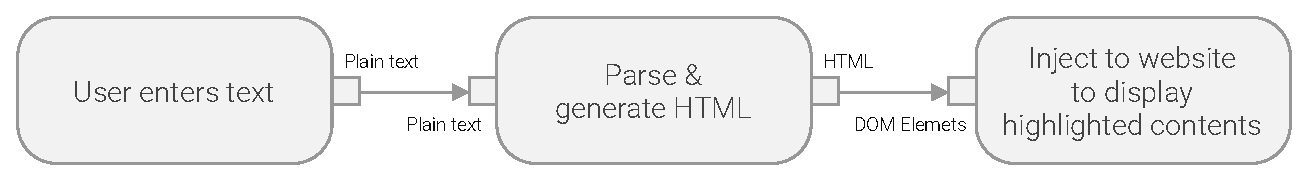
\includegraphics[width=\textwidth]{images/ace-codemirror-uml.eps}}
\caption{Rendering of highlighted source code in Ace and CodeMirror}
\label{fig:ace_rendering_uml}
\end{figure}


Web-based code editors like ''Ace'' and ''CodeMirror'' demonstrate that this is possible. They display syntax-highlighted source code editable by the user. The user seemingly writes inside the highlighted text and is also presented with a caret as well as the above mentioned components. In reality, the content inside the editor that a user sees is a regular part of the DOM---non-editable text, colored and formatted using HTML and CSS. When the user enters text, the input will be read with JavaScript. Based on the input Ace and CodeMirror generate HTML and add it to the editors contents, to show a properly syntax-highlighted representation (see figure~\ref{fig:ace_rendering_uml}). A \texttt{div} element that is styled to look like a caret is shown and moved with the user's keyboard and mouse input. The user's text input will be inserted at the according text offset. Amongst others, Ace and CodeMirror use other elements like \texttt{div}s to display a text selection and a \texttt{textarea} to fetch keyboard inputs, to recreate the behavior and capabilites of a native text input. Google's document editor uses similar techniques too.

%In reality, the user's input will be read with JavaScript and the code he or she sees is HTML generated based on this input to display syntax-highlighted text. Other components, like the caret and even the selection \texttt{div} elements, styled and positioned to mimick their native counterparts. 

%All this creates the illusion of a native text input.

%Many of the techniques to mimick a native text input like this can be found in web-based code editors like ''ACE'' or ''CodeMirror''.

Using tricks and \textit{faking} elements or behavior is common in web front end development. This applies to JavaScript as well as to CSS. For instance, long before CSS3 has been developed, techniques (often called ''hacks'') have been discussed on how to implement rounded corners without actual browser support. Only years later, this has become a standard. This not only enables features long before the creators of browsers implement them, this \textit{feedback} by the community of web developers also influences future standards. Encorporating feedback is a core philisophy of the WHATWG, the creators of HTML5.

Hacks are a necessity for an editor like this. The following sections will discuss each part of the editor and describe ideas, techniques and hacks that can be used for an effective implementation. In prior, we will discuss goals and principles that these techniques should be oriented towards as well as restrictions of browsers these techniqes must adapt to. % worst sentence ever

\section{Usage of HTML elements}

Ace, CodeMirror and Google's document editor shre similar concepts for imitating a native text input. For the caret, each of the editors create a \texttt{div} element, style it to make it look like a caret and move it when the user clicks in the text or uses his or her arrow keys. Each editor also uses \texttt{div} elements to display a text selection, styled to imitate the user's operating system's native selections. %In fact, there is hardly no alternative way

The concept to use HTML elements for the visible components of text editing is inevitable. Anything that can be seen on a website must exist in the DOM. The only deviation to this approach would be to resort a \texttt{canvas} element, as discussed above. The apporach to use HTML elements will be used for the implementation of this editor.

% Google, unlike Ace and CodeMirror displays a custom context menu. 

\section{Interaction with browser APIs}

Interaction with the browser must be well chosen. In some cases browser interaction can cause bugs and slow down performance while in some cases it can increase performance. The library should conform these rules:

\begin{enumerate} 
\item Minimize interaction with the DOM
\item Minimize interaction with unstable APIs
\item Use browser APIs if it improves performance or structure
\end{enumerate}

DOM operations can trigger a browser reflow\footnote{\url{https://developers.google.com/speed/articles/reflow}, last checked on 07/19/2015} which slows down the browser's performance. For this reason DOM operations should be avoided where possible.

Some APIs like the browser's \texttt{Range} or \texttt{Selection} interface are useful but known to be unstable. Libraries like Rangy try to tackle this by shimming parts of the interfaces. This requires complex methods and it is hard to account for possibly unknown bugs in the browsers' APIs. Ultimately this will also affect the library's file size. Instead of trying to fix native APIs, only as little as possible should be used. Instead of using possibly unstable APIs, pure JavaScript implementations should be used. Possibly unstable native APIs should only be used when it is inevitable.

Avoiding DOM operations and unstable APIs leads to a software architecture where the biggest part remains in its own business logic. Anything that can be implemented in pure JavaScript and does not cost performance or memory \textit{should} be implemented in pure JavaScript using own methods and data structues.

Facebook defined a similar goal for the user interface library React. React implements virtual DOM, an internal represenation of the actual DOM on which all operations should be performed, which in return does as little manipulation to the actual DOM as needed, to maximize performance. While the focus of this goal for this library is not solely performance, this part of it. However, there can be situations in which (even unstable) native browser methods may be faster than a JavaScript implementation. The text flow for instance should be left to the browser. There can also be cases in which a pure JavaScript implementation would be much more complex and would be at the expense of having a simple code structure. It must be decided in each particular case to use native and possible unstable APIs or a pure JavaScript implementation.

%Improving means it should be more explicit in what it does. The \texttt{bold} command of \texttt{execCommand} will manipulate the DOM to format text bold. It does not state in what how. Simple etc, what I have stated at Disadvantages of offering user interface components.

\section{Markup} 

The editor should be a ''good citizen'' in the ecosystem of other editors (see \refsubsec{subsec:noapi_dis_formatting}) and should generate valid markup, expressing a formatting semantically correct with as few tags as possible. The algorithm for creating markup must be able to work on any markup parsable by the browser and in return must generate predictable, \textit{simple} markup itself. It must not inject markup required for the internal workings of the editor\footnote{FirePad and Google' document editor inject markup for each text line, necessary for the internal functions of the editor}.


% dom operations could also be cached

\section{User interface components}

Most rich-text editors are implemented and distributed as user interface components. That means instead of only providing a library that offers methods to format the selected text and leaving the implementation of the user interface to the respective developer, most libraries are shipped as input fields with a default editor interface that is, at best, customizable.

This can be unfitting for many situations. The user interface of an editor highly depends on the software it will be integrated in. Within the software the interface may even vary depending on its specific purpose. For instance, a content management system may require an edtitor with a menubar offering many controls while a comment form on a blog requires only very little controls. Medium.com uses an interface that only shows controls when the user selects text and has no menubar at all. Assuming there are many implementations of editors that are in fact functional, it seems, choosing between editors is often just a choice of the desired ui. Customizing a ui can be just as complex as writing a ui from scratch. The latter affords to add HTML elememts and call JavaScript methods while both, customizing a user interface and writing a user interface from scratch require styling. In a worst case scenario, it can be more complex to customize an interface to specific needs then writing one from scratch and being able to define just the elements as they are required. That is why the library ''Type'' will be implemented and offered as a software library, rather than an editor and a user interface component.

%On a final note, until today, some rich-text editors use an iFrame to encapsulate the editor's contents and some don't. iFrame hat vor und nachteile. mit meiner library kann es jeder so machen, wie er/sie es will, weil es nur ne library ist.


\section{API}
\label{sec:api_design}
\label{sec:las_before_software_architecture}

\subsection{Conformity with HTML Editing APIs}

The library should be capable of any method implemented by HTML editing APIs. However the API can differ to improve they way it will be worked with.

\subsection{API Design}

% It can be much more fitting for developers to include a library that handles all text-input and -formatting operations while only providing a powerful API, leaving the ui to the developer. 

% While it can be much more fitting for developers to use an API to implement an
The API of this library must be \textit{well-designed}. That means it must be simple, effective and fit the developers' needs. The methods it offers should be simple in the sense that they conceal possibly complex tasks with understandable high-level concepts. They should be effective and fit the developers' needs in the sense that the API should be designed so that any requirement to of the developers should be matched with as little effort as possible. The API should create a workflow for developers that allows them to do what they want to do and is as easy to use and plausible as possible. jQuery is an example of encorporating an API conforming these principles.

The library's API will have two basic use cases. On the one hand, web developers must be enabled to implement rich-text editors with it. On the other hand, the library should offer interfaces for enabling web developers to extend the API and add features.

\paragraph{Extension}

For extension, web developers should have specific access to as many components and functions of the library, providing as much freedom and options as possible. This will include low-level access to components while control and explicitness is more imporant than simplicity. 

All components of Type will be implemented as classes. To provide as much capabilites as possible to other developers, all classes of Type will be exposed in a designated namespace. The classes should conform the best practices of object-oriented programming to support developers in extending the library. The class design should not only consider the specific needs of the core library but also potential use cases for other developers.

For example, with a designated class to show and move a caret, multiple carets can be instantiated for an extension that allows real-time collaboration with mutliple users. All available classes will be discussed in chapter \refchapter{ch:impl}.

\paragraph{Editor implementation}

For web developers implementing an editor (assuming the library offers all necessary features) the API should be designed to offer methods for the most common tasks related to rich text editing to allow fast and easy integration in a website. This should be high-level methods as compared to methods required for extending the library. Simplicity is more important than exact control over low-level behaviour. For implementing a rich-text editor the exposed methods should cover

\begin{enumerate}
\item Formatting and removing formats
\item Insertion
\item Deletion
\item Controlling the caret
\item Controlling the text selection
\item Controlling the clipboard
\item Controlling settings
\item Undo / redo commands
\end{enumerate}

\noindent jQuery demonstrates an effective and simple approach to API design, conforming the principles as discussed above. In jQuery all methods remain in a flat hierarchy within the root of a jQuery collection. Any method that is not a getter allows chainging and most methods are overloaded to allow passing various kinds of parameters, to determine what the function should do. Following these and the abovementioned principles, the components listed above can be expressed in 11 functions:

\begin{lstlisting}[language=JavaScript, caption=API for implementing a rich-text editor, label=lst:rich_text_api]
editor.caret([options, ...]);
editor.selection([options, ...]);
editor.insert([options, ...]);
editor.format([options, ...]);
editor.remove([options, ...]);
editor.settings([options, ...]);
editor.copy();
editor.cut();
editor.paste();
editor.undo();
editor.redo();
\end{lstlisting}

\noindent The functions in lines 1 through 6 can take various overloaded parameters to determine the specific action. The selection command, for instance, can be called with two numbers to draw a selection from one character offset to another (to draw a selection from characters 10 to 20 \code{editor.selection(10, 20);} can be called). It can also be called without passing parameters, to read the selection. \code{editor.selection();} would return the currently selected text as a string. A full API description can be found at table TODO.

%Applied to Type, this means

%As discussed in \refsubsec{subsec:flawed_api}, the HTML editing APIs, while being high-level and simple, still lack control and can be improved in that sense while still being simplified. As proposed in \refsubsec{subsec:adv_flawed_api}, to simplify the API and to increase control, all 17 formatting commands will be replaced with a single \code{format} method that accepts an \code{htmlString} compatible to jQuery.

%\noindent This will even account for cases where it is necessary to differenciate between an \code{i} element and an \code{em} element for semantical reasons.

\subsection{Handling use cases}

We can call programmers extending the library ''developers of the library'' and programmers using the library to implement editors ''users of the library''. To account for both use cases and maintain a clear software architecture and separation of concerns, all classes that provide functionality to the library must remain in a designated namespace which the library has access to. 

\begin{figure}[!htb]
\centering
\makebox[\textwidth]{\includegraphics[width=\textwidth]{images/concept-sep-use-cases.pdf}}
\caption{UML of the Type library and its internally used classes (exceperpt)}
\label{fig:type_uml_excerpt}
\end{figure}

The library itself will be exposed as a class to the global namespace with the name ''Type''. It can be instantiated and then provides an own API, the high-level methods, for implementing a rich-text editor.

%Ursprünglich API und Codestruktur an window.execCommand orientiert, das ist aber doof.
%Bessere (weil präzisere) API mit mehr Möglichkeiten als der contentEditable scheiss
%für Programmierer und für 2 anwendungsfälle:
%einen editor bauen
%type mit plugins erweitern
%für beides gibt es die passenden Funktionen, das eine einfach und schlau, das andere präzise
%Deswegen werden auch alle Module, alle Klassen exponiert aber es gibt eine eigene API nach jQuery konzept
%Type kommt mit bestimmten Kernmodulen die fuer Textbearbeitung essenziell sind. Aber an dieser Stelle laesst sich Type um weitere Module anhand einer KOnvention (erweitern des Type Objekts) erweitern.
%Ursprünglich API und Codestruktur an window.execCommand orientiert, das ist aber doof.

%The library shall give other developers as much freedom as possible, meaning other developer should use the library as they see it fit and not the other way around, should try to conform the needs of the library.


\part{\ Implementation}
\label{part:implementation}

\chapter{All}
\label{ch:impl_all}

%!TEX root = ../../thesis.tex

\chapter{Evaluation}
\label{ch:evaluation}


\section{Features}

It can be integrated in any website to allow other developers

The resulting editor of this thesis demonstrates a way to implement a rich-text editor on the web without using HTML editing APIs. With \textit{Type}, web developers can turn any elements into an editable sections in which:

%The resulting editor of this thesis is capable of basic rich-text editing including real-time collaboration. 

\begin{itemize}
\item Text can be written and removed.
\item Text can be formatted.
\item The caret can be controlled.
\item The text selection can be read and controlled.
\item An editor can be connected to an Etherpad server for real-time collaboration alongside Etherpad's own clients
\item Changes can be undone and redone accounting for multiple input sources (like Etherpad)
\item An editor can be interacted with like a native input field
\end{itemize}


 
The library can be extended and improved by third-party developers.
 
Third-party developers can extend
 - ecosystem for extension
 - control input
 - control pasting
 
\section{MVC \& Document model}

Towards the end of this thesis, Marijn Haverbeke, author of CodeMirror, started a crowd-funding campaign for supporting him to build a rich-text editor that does not rely on HTML editing APIs---called ProseMirror---just like library of this thesis. As discussed in \refsection{sec:mvc_architecture}, \textit{Type} does not rely on an architecture that abstracts the contents of the editor from the DOM. ProseMirror, by contrast, takes this approach. This restricts working with the editor to the capabilities of the internal model of the document and might make extending the editor complicated. On the other hand, it allows for a very stable rendering of the contents and (as discussed) switching between HTML or Markdown output. It is good to see both approaches being realized. By contrasting both approaches in a practical manner it might be easier to decide which approach is better for which purposes.

\chapter{Outlook}
\label{ch:outlook}






\section{Evaluation notizen}

There are some things that need to be done
 - Bugs, tests
 - Mobile support
 - BiDi \& IME support
 - A more profound model to sync with etherpad
 - trigger more events
 - images, tables, lists




\section{Mobile Support}

It's technically there, it must be tested properly


\subsection{BiDi \& IME support}

http://marijnhaverbeke.nl/blog/cursor-in-bidi-text.html

http://marijnhaverbeke.nl/blog/browser-input-reading.html 

https://en.wikipedia.org/wiki/Input\_method


\section{Development / Meta}
Crockford style is a bad idea. 
I will change it to Standard or Airbnb 
\url{https://github.com/airbnb/javascript/tree/master/es5}


\section{Outlook}

Over time, the bugs of HTML editing APIs will decrease. Its clipboard capabilities are on the way to be expanded. The API still is still limited and needs a revision. It is even imaginable to rethink the way \code{contenteditable} works. Editors that, for instance, implement layouting, like Google's document editor, still cannot be implemented with the way HTML Editing APIs are designed.

To allow a transition from current HTML editing APIs and an interface with a cleaner and richer functionality, it is thinkable to introduce a new ''class'' alongside the old API. This has been done with other functionality, for example mal aus MDN raussuchen. This way the old API can die gracefully while web developers slowly adopt. It can be hoped that if the API is much better, the adoption will happen quickly.


As discussed in \refsubsec{subsec:edit_api_adv_thir_party_lang} my design as a library with a super duper api allows implementing highlighting for other languages like bb code or markdown. \textit{There should be a part in CONCEPT that explains this idea, either explaining its made for extensibility or in how cool my api is i mean the design as a lib and not as an editor is}


besseres undo durch erkennen von ganzen worten (wenn man leerzeichen und so drückt)

Events zu allen gelegenheuten triggern für andere developer


DOCH document model benutzen weil der shit von prosemirror einfach so geil ist.

Auf der anderen Seite ist so was wie der Medium editor mit meiner Version viel besser

\part{Evaluation}
\label{part:evaluation}

%!TEX root = ../../thesis.tex

\chapter{Evaluation}
\label{ch:evaluation}


\section{Features}

It can be integrated in any website to allow other developers

The resulting editor of this thesis demonstrates a way to implement a rich-text editor on the web without using HTML editing APIs. With \textit{Type}, web developers can turn any elements into an editable sections in which:

%The resulting editor of this thesis is capable of basic rich-text editing including real-time collaboration. 

\begin{itemize}
\item Text can be written and removed.
\item Text can be formatted.
\item The caret can be controlled.
\item The text selection can be read and controlled.
\item An editor can be connected to an Etherpad server for real-time collaboration alongside Etherpad's own clients
\item Changes can be undone and redone accounting for multiple input sources (like Etherpad)
\item An editor can be interacted with like a native input field
\end{itemize}


 
The library can be extended and improved by third-party developers.
 
Third-party developers can extend
 - ecosystem for extension
 - control input
 - control pasting
 
\section{MVC \& Document model}

Towards the end of this thesis, Marijn Haverbeke, author of CodeMirror, started a crowd-funding campaign for supporting him to build a rich-text editor that does not rely on HTML editing APIs---called ProseMirror---just like library of this thesis. As discussed in \refsection{sec:mvc_architecture}, \textit{Type} does not rely on an architecture that abstracts the contents of the editor from the DOM. ProseMirror, by contrast, takes this approach. This restricts working with the editor to the capabilities of the internal model of the document and might make extending the editor complicated. On the other hand, it allows for a very stable rendering of the contents and (as discussed) switching between HTML or Markdown output. It is good to see both approaches being realized. By contrasting both approaches in a practical manner it might be easier to decide which approach is better for which purposes.

\chapter{Outlook}
\label{ch:outlook}






\section{Evaluation notizen}

There are some things that need to be done
 - Bugs, tests
 - Mobile support
 - BiDi \& IME support
 - A more profound model to sync with etherpad
 - trigger more events
 - images, tables, lists




\section{Mobile Support}

It's technically there, it must be tested properly


\subsection{BiDi \& IME support}

http://marijnhaverbeke.nl/blog/cursor-in-bidi-text.html

http://marijnhaverbeke.nl/blog/browser-input-reading.html 

https://en.wikipedia.org/wiki/Input\_method


\section{Development / Meta}
Crockford style is a bad idea. 
I will change it to Standard or Airbnb 
\url{https://github.com/airbnb/javascript/tree/master/es5}


\section{Outlook}

Over time, the bugs of HTML editing APIs will decrease. Its clipboard capabilities are on the way to be expanded. The API still is still limited and needs a revision. It is even imaginable to rethink the way \code{contenteditable} works. Editors that, for instance, implement layouting, like Google's document editor, still cannot be implemented with the way HTML Editing APIs are designed.

To allow a transition from current HTML editing APIs and an interface with a cleaner and richer functionality, it is thinkable to introduce a new ''class'' alongside the old API. This has been done with other functionality, for example mal aus MDN raussuchen. This way the old API can die gracefully while web developers slowly adopt. It can be hoped that if the API is much better, the adoption will happen quickly.


As discussed in \refsubsec{subsec:edit_api_adv_thir_party_lang} my design as a library with a super duper api allows implementing highlighting for other languages like bb code or markdown. \textit{There should be a part in CONCEPT that explains this idea, either explaining its made for extensibility or in how cool my api is i mean the design as a lib and not as an editor is}


besseres undo durch erkennen von ganzen worten (wenn man leerzeichen und so drückt)

Events zu allen gelegenheuten triggern für andere developer


DOCH document model benutzen weil der shit von prosemirror einfach so geil ist.

Auf der anderen Seite ist so was wie der Medium editor mit meiner Version viel besser